


\chapter{Logical Modelling}{“All models are wrong, but some are useful.”}\label{chapLogicalModelling}

This section is about math. Nevertheless, before deepening into math, it is necessary to mention the Logic, another important branch of science deeply connected with math. The Logic was the main character of the philosophical debate in ancient Greece. Aristotle was the first to set the rules of the Logic as we study nowadays \cite{Aristoteles}. \par

Today we study the Logic by using the truth table and the logical operator (i.e. $AND$, $OR$, $NOT$). These simple operations on zero and ones are performed on any CPU allowing from simple calculations to the moon landing, to machine learning and artificial intelligence. Every input or output of a computer is processed by using the rules of the logic. \par

Logical modelling is crucial for all the STEM disciplines (science, technology, engineering and mathematics) to identify a deterministic connection between the input and the output of a phenomenon. Logic permits to STEM researchers to build models based on their intuitions. These models can be validated or not by using math and statistics. Nevertheless, it is necessary to remember that all models are wrong. Models approximate reality, but they are not reality. For this reason, they are wrong.\par

Models help to understand how reality works. If you can understand reality, you can control, and change it. This fact is actual in the field of logistics and operations, whose environment involves thousands of resources, assets, goods and tasks. In this chapter, we use the logic to model and connect these entities aiming at the understanding of complex operational environments.\par 

\section{Business Process Model and Notation} \label{secBPMN}
Literature introduces many notations for modelling a business process. In this work, we introduce the Business Process Model and Notation (BPMN) that results adequate, when applied to the modelling of logistics and operational processes \cite{OMG1998}. The BPMN uses a number of predefined symbols to model entities, flows, resources and activities of any business process. The full notation requires hundred of pages of details, but the main elements (see Figure \ref{fig_BPMN}) are three \cite{White2004}:

\begin{itemize}
    \item Event: it is represented by a circle and is something that “happens” during a business process. These Events affect the flow of the process and usually have a cause (trigger) or an impact (result). 
    \item Activity: it is represented by a rounded-corner and is a generic term for work that company performs. 
    \item Gateway: it is represented by a diamond and is used to control the divergence and convergence of Sequence Flow as a logic gate.

\end{itemize}

% INSERT fig_bpmn
\begin{figure}[hbt!]
\centering
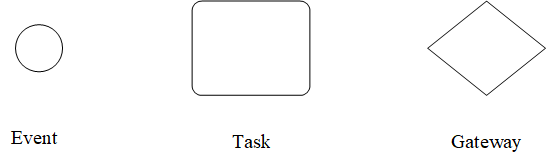
\includegraphics[width=0.8\textwidth]{SectionLetsMath/logicalModelling_figures/fig_BPMN.png}
\captionsetup{type=figure}
\caption{Main elements of a BPMN.}
\label{fig_BPMN}
\end{figure}

The following sections of this work identify the resources, asset, tasks and goods to associate with each of these elements. Figure \ref{fig_es_BPMN} illustrates an example of a BPMN to describe the operations of a port terminal.\par 

% INSERT fig_es_bpmn
\begin{landscape}
\thispagestyle{empty}
\begin{figure}[hbt!]
\centering
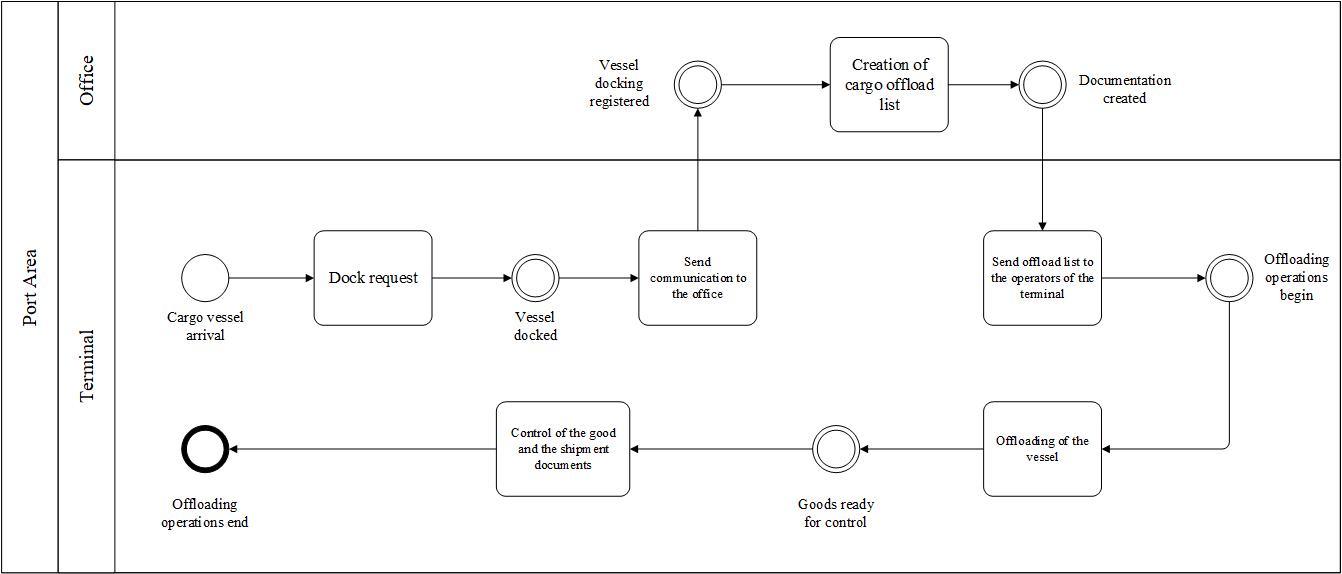
\includegraphics[width=1.3\textwidth]{SectionLetsMath/logicalModelling_figures/fig_es_BPMN.png}
\captionsetup{type=figure}
\caption{an example of a BPMN applied to the logistics of a port terminal.}
\label{fig_es_BPMN}
\vfill
\end{figure}
\end{landscape}

An additional logistic feature of the BPMN is represented by the possibility of georeferencing tasks and events. Using this method, the physical location of each activity is identified. In addition, it is possible to annotate the responsible of the activity. The BMN allows tracking the physical and information flows of logistics operations qualitatively, by introducing logical rules on the events and gateways leading to the tasks.

%\clearpage
\bibliographystyle{ieeetr}
\bibliography{SectionLetsMath/logicalModelling_ref}
